\section{\large Exercises}

\begin{exer}
    Find the values of $m$ and $n$ if $\Delta ABC \cong \Delta QRP$ by $LA \cong$
    \begin{figure}[H]
        \center
        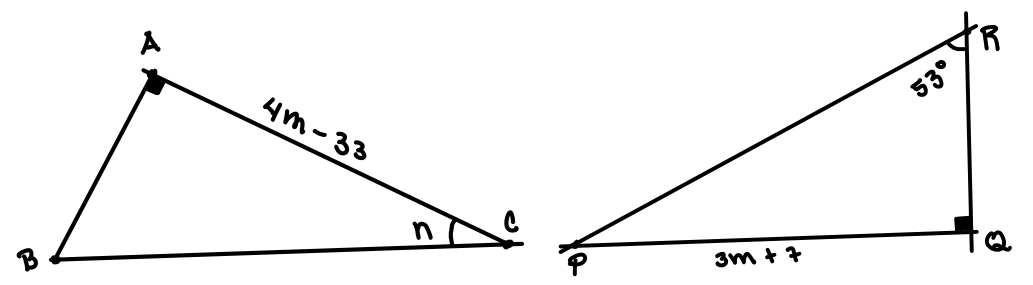
\includegraphics[width=15cm]{content/img1.png}
    \end{figure}
\end{exer}
\vspace{4cm}

\begin{exer}
    Explain textually what a perpendicular bisector is.
    Then, make two drawings; one where a perpendicular bisector is shown and another where it is not.
\end{exer}

\newpage

\begin{exer}
    Find the orthocenter of $\Delta ABC$ in the following figure.
    Then, explain what relationship exists between the circumference $\omega$ and the orthocenter of $\Delta ABC$.
    \begin{figure}[H]
        \center
        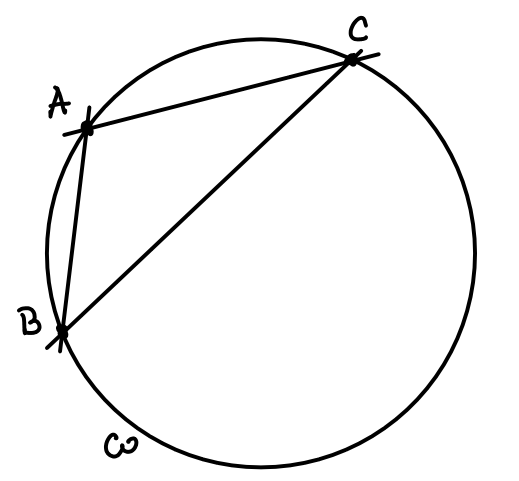
\includegraphics[width=6cm]{content/img2.png}
    \end{figure}
\end{exer}

\vspace{2cm}
\begin{exer}
    Find each of the following if $U, V$ and $W$ are the midpoints of $\overline{RS}$, $\overline{ST}$ and $\overline{TR}$.
    \begin{multicols}{2}
        \begin{figure}[H]
            \center
            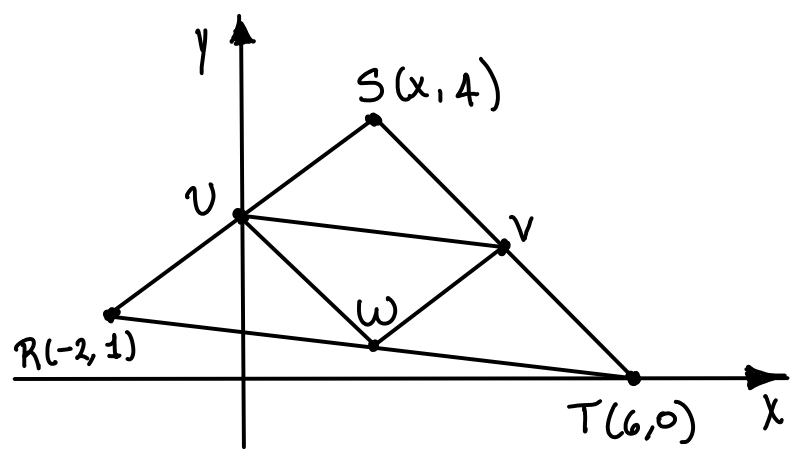
\includegraphics[width=8.5cm]{content/img3.png}
        \end{figure}
        \begin{enumerate}
            \item $\angle SUV$
            \item $\angle UVW$
            \item $\overline{RS}$
            \item $\overline{UV}$
            \item the coordinate of $W$
            \item the x-coordinate of $S$
            \item the coordinate of $V$
        \end{enumerate}
    \end{multicols}
\end{exer}